%   % !TEX root = ../../VIII,3_Rahmen-TeX_8-1.tex
%
%   Band VIII, 3 N.~??A32
%   Signatur/Tex-Datei: LH_35_09_16_019
%   RK-Nr. 41178 (mit RK 41179 zusammen)
%   Überschrift: [De funibus inaequaliter tensis]
%   Modul: Mechanik / AEF
%   Datierung: [nach Mitte März 1683]
%   WZ: Keins
%   SZ: Keins
%   Bilddateien (PDF): LH_35_09_16_019_d1; LH_35_09_16_019_d2 (insgesamt: zwei)
%
%
\selectlanguage{ngerman}%
\frenchspacing%
%
\begin{ledgroupsized}[r]{120mm}
\footnotesize
\pstart
\noindent\textbf{Überlieferung:}
\pend
\end{ledgroupsized}
\begin{ledgroupsized}[r]{114mm}
\footnotesize
\pstart \parindent -6mm
\makebox[6mm][l]{\textit{L}}%
Aufzeichnung:
LH~XXXV~9,~16 Bl.~19.
Ein Blatt 8\textsuperscript{o}.
Zwei Seiten.
Bl.~19~v\textsuperscript{o} überliefert ferner, gegenläufig und überschrieben, den Anfang eines Briefkonzeptes von Leibnizens Hand,
dessen Adressat sich nicht eindeutig ermitteln lässt: % } \lbrack/\rbrack\ \textit{
\textit{WohlEdler Vester,\protect\index{Sachverzeichnis}{Vester} % \\
insonders Hochgeehrter H. % \\
Mein schreiben aus Braun% -\\
schweig\protect\index{Ortsregister}{Braunschweig} wird verhoffentlich % \\
zu recht geliefert worden % \\
seyn. Anjezo muß % \\
selbigen abermahl bemühen. % \\
Ich habe anhehr eilen müßen % \\
weilen ich verstanden, daß % \\
man kunftigen Montag % \\
alhier aufbrechen will; und % \\
ich noch zuvor ein und anders % \\
alhier zu Verrichten habe. % \\
Unter anderm} \lbrack\textit{Text bricht ab.}\rbrack\
\pend
\end{ledgroupsized}
%
\vspace{5mm}
\begin{ledgroup}
\footnotesize
\pstart
\noindent\textbf{Datierungsgründe:}
In dem Brieffragment, das auf demselben Träger wie die Aufzeichnung N.~22 mit überliefert ist, erwähnt Leibniz ein früheres \textit{Schreiben aus Braunschweig}, das er offenbar an seinen (nicht ermittelten) Adressaten gesendet hatte.
Von einem Besuch bei seinem Oheim J.~Strauch\protect\index{Namensregister}{\textso{Strauch}, Johann 1612(?)\textendash1679(?)} im März 1664 abgesehen, hielt sich Leibniz erstmals vom 10. bis zum 13. März 1683 in Braunschweig auf, als er dort Anton Ulrich von Wolfenbüttel\protect\index{Namensregister}{\textso{Anton Ulrich} v. Wolfenbüttel; Herzog v. Braunschweig-Lüneburg 1685\textendash1714} wahrscheinlich kennenlernte (\textit{Chronik}, S.~8; 70\cite{01236}).
Hieraus lässt sich der Terminus post quem der Datierung erschließen:
Da das Brieffragment schon vorgelegen hatte, als die Aufzeichnung N.~22 verfasst wurde, kann diese letztere nicht vor Mitte März 1683 entstanden sein.
\pend%
\pstart%
Ein Terminus ante quem lässt sich hingegen nach heutigem Wissensstand nicht eindeutig bestimmen.
Freilich spricht einiges dafür, die Aufzeichnung chronologisch noch in die Achtziger Jahre zu verorten (zwischen Mitte März 1683 und der Italienreise im Herbst 1687).
Zunächst beschäftigte sich Leibniz seit den frühen Achtziger Jahren intensiv mit Themen der Elastizität und insbesondere mit dem mechanischen Verhalten gespannter Saiten oder Seile, wie zahlreiche Texte in diesem Band zeigen (etwa N.~8; 9; 10).
Dies lässt sogar die Vermutung zu, dass N.~22 nicht viel später als Mitte März 1683 entstanden sein dürfte, d.h. etwa zu der Zeit, als inhaltlich verwandte Texte wie N.~14\textsubscript{3}, 14\textsubscript{7} und 17 verfasst wurden.
% ;die Vermutung wird auch dadurch bekräftigt, dass kein weiterer Aufenthalt Leibnizens in Braunschweig bis Ende August/Anfang September 1690 belegt ist (\textit{Chronik}, S.~105\cite{01236}).
Auch die im Brieffragment verwendete Anrede \textit{Vester} kommt am häufigsten \textendash\ sofern der Zustand der Überlieferung eine Einschätzung ermöglicht \textendash\ in Briefen vor, die Leibniz während der Achtiziger Jahre in amtlichen bzw. förmlichen Kontexten schrieb.
So findet sich etwa die Formel \textit{Wohl\-Edler Vester insonders Hochgeehrter Herr} (allenfalls leicht variiert) u.a. in seinen Briefen an:
F.\,W. Leidenfrost
(Ende Juli 1680, \textit{LSB} I,~3 N.~46;\cite{01325}
Mitte Januar 1682, ebd. N.~112;\cite{01326}
6.? April 1688, \textit{LSB} I,~5 N.~33);\cite{01327}%
\protect\index{Namensregister}{\textso{Leidenfrost}, Friedrich Wilhelm, nach 1648\textendash1703}
%
C.~Wichmann
(5./15. Mai 1682, \textit{LSB} I,~3 N.~135;\cite{01328}
29. September/9. Oktober 1682, ebd. N.~165);\cite{01329}%
\protect\index{Namensregister}{\textso{Wichmann}, Christoph, gest. 1690}
%
P.~Marci
(20./30.~März 1685; \textit{LSB} I,~4 N.~417);\cite{01330}%
\protect\index{Namensregister}{\textso{Marci}, Polycarp 1654\textendash1724}
%
P.\,P. Metzger
(1685?; \textit{LSB} I,~4 N.~457)\cite{01331}%
\protect\index{Namensregister}{\textso{Metzger}, Peter Paul 1639\textendash1699}
%
oder G.~Mennichen
(Ende Januar 1687; \textit{LSB} I,~4 N.~267).\cite{01332}%
\protect\index{Namensregister}{\textso{Mennichen}, Georg gest.\ nach 1687}
%
Leidenfrosts Brief an Leibniz vom 12. (22.) März 1683 (\textit{LSB} I,~3 N.~187)\cite{01333}
könnte möglicherweise sogar das erwähnte \textit{schreiben aus Braunschweig} beantwortet haben.
Eine sichere Zuordnung des Brieffragments ergibt sich aus diesen Umständen jedoch nicht.
Vielmehr ist festzustellen, dass die Formel \textit{WohlEdler Vester insonders Hochgeehrter Herr} 
sporadisch auch in späteren Briefen Leibnizens vorkommt,
etwa an P.~Marci (27. März/7. April 1691; \textit{LSB} I,~6 N.~247)\cite{01334}
oder D.~Flach (5./15.~Juni 1693; \textit{LSB} I, Supplementband Harz-Bergbau, N.~28).\cite{01335}%
\protect\index{Namensregister}{\textso{Flach}, Daniel, gest. 1694}
%
Aufgrund dieser späteren Vorkommnisse und unter Berücksichtigung der zahlreichen Aufenthalte Leibnizens in Braunschweig\protect\index{Ortsregister}{Braunschweig} und Wolfenbüttel\protect\index{Ortsregister}{Wolfenbüttel} seit 1690 ist eine Datierung der Aufzeichnung N.~22 auf die Zeit nach der Italienreise nicht auszuschließen.
\pend
\end{ledgroup}
%
\selectlanguage{latin}%
\frenchspacing%
%
%
% \vspace{8mm}
\newpage%
\pstart%
\noindent%
\normalsize%
%
%
%  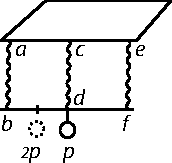
\includegraphics[width=0.2\textwidth]{gesamttex/edit_VIII,3/images/LH_35_09_16_019_d1.pdf}\\
%  \lbrack\textit{Fig.~1}\rbrack\
%
%
\lbrack19~r\textsuperscript{o}\rbrack\ %%%% Blatt 19r
\edtext{}{%
\lemma{\textit{Am oberen Rand:}}\Afootnote{%
Haec subtilissima et magni momenti.
(\protect\vphantom)%
Quae sub NB~\astrosun, re discussa pro veris habenda.%
\protect\vphantom()%
\textsuperscript{\lbrack a\rbrack}\vspace{0.5em}%
\newline%
{\footnotesize%
\textsuperscript{\lbrack a\rbrack}~%
(\protect\vphantom)Quae \lbrack...\rbrack\ habenda.\protect\vphantom()\,:
Siehe die entsprechende Randbemerkung auf S.~\pageref{LH_35_09_16_019r_rndbmrkg_NBsun}.\vspace{-6mm}}}}%
%
%
Ex \edtext{laqueari\protect\index{Sachverzeichnis}{laquear}
seu tecto\protect\index{Sachverzeichnis}{tectum} \textit{ace}}{%
\lemma{laqueari \lbrack...\rbrack\ \textit{ace}}\Cfootnote{%
Siehe das Diagramm \lbrack\textit{Fig.~1}\rbrack.}}
%
pendeant tres funes\protect\index{Sachverzeichnis}{funis pendens}
aeque longi et crassi \textit{ab}, \textit{cd},
%
\edtext{\textit{ef} per quorum extremitates inferiores}{%
\lemma{\textit{ef}}\Bfootnote{%
\textit{(1)}~per
\textit{(a)}~\textlangle eo\textrangle\
\textit{(b)}~infer
\textit{(2)}~per quorum extremitates inferiores%
~\textit{L}}}
%
transeat transversus baculus\protect\index{Sachverzeichnis}{baculus transversus} \textit{bdf}
ex quo pendeat
%
\edtext{pondus\protect\index{Sachverzeichnis}{pondus pendens} \textit{p}.
His positis si pondus \textit{p} sit in medio itemque funis \textit{cd},
funes quidem \textit{ab} et \textit{ef}}{%
\lemma{pondus}\Bfootnote{%
\hspace{-0,5mm}\textit{p}.
\textit{(1)}~His
\textit{(2)}~Si pondus \textit{p},
\textit{(a)}~\textlangle et funis\textrangle\
\textit{(b)}~funes \textit{ab}
\textit{(c)}~si
\textit{(3)}~His positis \lbrack...\rbrack\ \textit{ab} et \textit{ef}%
~\textit{L}}}
%
aequaliter
%
\edtext{\lbrack ten\-den\-tur\rbrack,}{%
\lemma{tendi}\Bfootnote{%
\textit{L~ändert Hrsg.}}}
%
sed et funis \textit{cd} tantundem tendetur,\protect\index{Sachverzeichnis}{funis tensus}
nisi in quantum baculus\protect\index{Sachverzeichnis}{baculus transversus} \textit{bdf} curvabitur in medio.
Nam si rigidus ponatur,
aut non aut aequaliter ubique descendet,
ideoque et aequaliter ubique funes tendet,
quare falsum est
%
\edtext{quod ajunt}{%
\lemma{quod ajunt}\Cfootnote{%
Vgl. etwa
\protect\index{Namensregister}{\textso{Wallis} (Wallisius), John 1616\textendash1703}%
J.~\textsc{Wallis}, \textit{Mechanica}, pars~III, cap.~VI, prop.~V
(London 1671\textendash1672, Bd.~II, S.~579f.;
\textit{WO}~I, S.~946).\cite{00301}\cite{01008}
Leibniz hatte in Paris die Stelle exzerpiert:
\textit{LSB} VIII,~2 N.~8, S.~71.8\textendash15.\cite{01343}}}
%
propiorem centro gravitatis,\protect\index{Sachverzeichnis}{centrum gravitatis}
ut hoc loco funem \textit{cd},\protect\index{Sachverzeichnis}{funis tensus}
magis gravari.
Verum si pondus \textit{p}\protect\index{Sachverzeichnis}{pondus tendens}
ponatur inter \textit{b}
%
\edtext{et \textit{d} in loco \textit{{\scriptsize 2}p}
tunc funis \textit{ab}
(\protect\vphantom)%
omittamus nunc funem \textit{cd}%
\protect\vphantom()
magis \lbrack gravabitur\rbrack\ 
quam funis \textit{ef}.}{%
\lemma{et \textit{d}}\Bfootnote{%
\textit{(1)}~funes
\textit{(2)}~in loco \textit{{\scriptsize2}p} tunc
\textit{(a)}~funes
\textit{(b)}~funis \textit{ab}
\textit{(aa)}~et \textit{cd}
\textit{(bb)}~(\protect\vphantom)omittamus nunc funem \textit{cd}\protect\vphantom() magis
\textbar~gravabuntur \textit{ändert Hrsg.}~%
\textbar\ quam funis \textit{ef}.%
~\textit{L}}}
%
Nam variis modis baculus transversus\protect\index{Sachverzeichnis}{baculus transversus}
cum annexo pondere\protect\index{Sachverzeichnis}{pondus annexum} descendere potest,
uno directo, ita ut ubique descendat aequaliter,\protect\index{Sachverzeichnis}{descensus directus}
et secundum hunc modum aequaliter tenderentur funes;\protect\index{Sachverzeichnis}{funis tensus}
altero circulari, eoque rursus duplici,\protect\index{Sachverzeichnis}{descensus circularis}
uno nempe ut circa centrum \textit{b}\protect\index{Sachverzeichnis}{centrum}
moveatur baculus \textit{bdf},\protect\index{Sachverzeichnis}{baculus transversus}
altero ut idem moveatur circa centrum \textit{f}.\protect\index{Sachverzeichnis}{centrum}
Hoc autem postremo modo maxime facilis redditur descensus,\protect\index{Sachverzeichnis}{descensus circularis}
cum ita
%
\edtext{vis\protect\index{Sachverzeichnis}{vis tendens}
in funem \textit{ab} maxime impendatur\protect\index{Sachverzeichnis}{vis impendens}
quae alias impenderetur in ambos \textit{ab} et \textit{ef}.}{%
\lemma{vis}\Bfootnote{%
\textit{(1)}~tota
\textit{(2)}~in
\textit{(a)}~duos tales funes
\textit{(aa)}~impendatur
\textit{(bb)}~\textit{ab}, \textit{ef}
\textit{(b)}~funem \textit{ab} \lbrack...\rbrack\ alias impenderetur
\textit{(aa)}~in ambos \textit{ab} \textit{cd}
\textit{(bb)}~in ambos \textit{ab} et \textit{ef}.%
~\textit{L}}}
%
\hspace{0.2mm}Difficile \hspace{0.2mm}tamen \hspace{0.2mm}est \hspace{0.2mm}determinare
\hspace{0.2mm}quantum \hspace{0.2mm}quisque \hspace{0.2mm}funis \hspace{0.2mm}debeat \hspace{0.2mm}tendi.\protect\index{Sachverzeichnis}{funis tensus}
\pend
  \vspace{1.5em}%
  \centerline{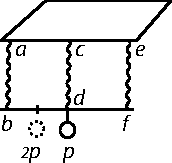
\includegraphics[width=0.20\textwidth]{gesamttex/edit_VIII,3/images/LH_35_09_16_019_d1.pdf}}% \hspace*{-55mm}
  \vspace{0.5em}%
  \centerline{\lbrack\textit{Fig.~1}\rbrack}% \hspace*{-55mm}
  \label{LH_35_09_16_019r_Fig.1}%
\newpage
\pstart
\noindent
Sane summa omnium tensionum\protect\index{Sachverzeichnis}{summa tensionum} tanta esse debet
quanta erat antea cum pondus\protect\index{Sachverzeichnis}{pondus tendens} esset in medio,
eadem enim vis\protect\index{Sachverzeichnis}{vis tendens} quae
%
\edtext{ante,
eandem producet effectus quantitatem,\protect\index{Sachverzeichnis}{quantitas effectus}}{%
\lemma{ante,}\Bfootnote{%
\textit{(1)}~eundem producet effectum\protect\index{Sachverzeichnis}{effectus}
\textit{(2)}~eandem producet effectus quantitatem,%
~\textit{L}}}
%
deinde non potest dici totam vim%
\protect\index{Sachverzeichnis}{vis tendens}%
\protect\index{Sachverzeichnis}{vis impendens}%
\protect\index{Sachverzeichnis}{vis tota}
%
\edtext{impendi soli funi \textit{ab},}{%
\lemma{impendi}\Bfootnote{%
\textit{(1)}~solis duobus funibus \textit{ab} et \textit{cd}
\textit{(2)}~soli funi \textit{ab},%
~\textit{L}}}
%
nam sciendum
%
\edtext{est illum aliquantum tensum}{%
\lemma{est}\Bfootnote{%
\textit{(1)}~illos aliquantum tensos
\textit{(2)}~illum aliquantum tensum%
~\textit{L}}}
%
magis resistere quam funem \textit{ef} omnino nondum
%
\edtext{tensum,\protect\index{Sachverzeichnis}{funis tensus}
et ita hac differentia situs differentiam\protect\index{Sachverzeichnis}{differentia situs} compensari.}{%
\lemma{tensum,}\Bfootnote{%
\textit{(1)}~licet alias com
\textit{(2)}~et 
\textit{(3)}~et ita \lbrack...\rbrack\ differentiam compensari.%
~\textit{L}}}
%
Pondere\protect\index{Sachverzeichnis}{pondus tendens} ergo sito in \textit{{\scriptsize 2}p},
eousque
%
\edtext{plus tendetur funis \textit{ab}}{%
\lemma{plus}\Bfootnote{%
\textit{(1)}~tendentur funes \textit{ab}, \textit{cd}
\textit{(2)}~tendetur funis \textit{ab}%
~\textit{L}}}
%
quam funis \textit{ef}\protect\index{Sachverzeichnis}{funis tensus}
%
\edtext{donec motui ponderis directo vel etiam circa centrum \textit{b}}{%
\lemma{donec}\Bfootnote{%
\textit{(1)}~motibus
\textit{(2)}~motui ponderis
\textbar~directo vel etiam \textit{erg.}~%
\textbar\ circa centrum \textit{b}%
~\textit{L}}}
%
minus resistat funis \textit{ef}
quam motui circa centrum \textit{f} resistit funis \textit{ab}.%
\protect\index{Sachverzeichnis}{funis tensus}
Res autem accurate sic poterit determinari,\protect\index{Sachverzeichnis}{res determinata}
ut pondus \textit{p}\protect\index{Sachverzeichnis}{pondus tendens}
eo descendat, quo longissime potest
eadem manente summa tensionum.%
\protect\index{Sachverzeichnis}{tensio funis}%
\protect\index{Sachverzeichnis}{summa tensionum}%
\edtext{\label{LH_35_09_16_019r_rndbmrkg_NBsun}}{%
\lemma{\textit{Am Rand, quer:}}\Afootnote{%
NB~\astrosun\
Pondus tantundem descendit quantum ante,\protect\index{Sachverzeichnis}{pondus tendens}
summa tensionum eadem quae ante,\protect\index{Sachverzeichnis}{summa tensionum}
funium autem tensiones sunt reciproce\protect\index{Sachverzeichnis}{tensio funis}
ut distantiae a centro gravitatis.\protect\index{Sachverzeichnis}{distantia a centro gravitatis}
Ex his tribus res determinatur.\protect\index{Sachverzeichnis}{res determinata}
NB~\astrosun}}%
%
\pend%
%
%
%%
%%  \newpage
%  \vspace{-9.0em}%
%  \centerline{\hspace*{55mm}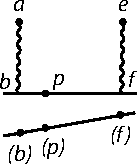
\includegraphics[width=0.15\textwidth]{gesamttex/edit_VIII,3/images/LH_35_09_16_019_d2.pdf}}%
%  \vspace{0.5em}%
%  \centerline{\hspace*{55mm}\lbrack\textit{Fig.~2}\rbrack}% \hspace*{16mm}
%  \label{LH_35_09_16_019v_Fig.2}%
%  \vspace{1.5em}%
%%
%
\pstart%
\edtext{Itaque
%
\lbrack19~v\textsuperscript{o}\rbrack\ %%%% Blatt 19v
%
si summa tensionum\protect\index{Sachverzeichnis}{summa tensionum} possibilis ponatur esse data,
et
\edtext{onus\protect\index{Sachverzeichnis}{onus} seu trabs \textit{bpf}\protect\index{Sachverzeichnis}{trabs}
descendat ad \textit{(b)(p)(f)}}{%
\lemma{onus \lbrack...\rbrack\ \textit{(b)(p)(f)}}\Cfootnote{%
Siehe das Diagramm \lbrack\textit{Fig.~2}\rbrack.}}
quaeritur,}{%
\lemma{Itaque}\Bfootnote{%
\textit{(1)}~erit \lbrack19~v\textsuperscript{o}\rbrack\
\textit{(2)}~si summa \lbrack...\rbrack\ esse data,
\textit{(a)}~quaeritur
\textit{(b)}~et onus \lbrack...\rbrack\ \textit{(b)(p)(f)} quaeritur,%
~\textit{L}}}
%
ubi debeat esse punctum \textit{(p)}
et quis angulus\protect\index{Sachverzeichnis}{angulus obliquitatis} obliquitatis rectae \textit{(b)(p)(f)};
et quidem differentiarum inter rectas \textit{ab} et \textit{a(b)},
item rectas \textit{ef} et \textit{e(f)}
summa debet aequari summae tensionum datae.\protect\index{Sachverzeichnis}{summa tensionum}
%
\edtext{(\protect\vphantom)%
Hinc sequitur summam $\textit{a(b)}+\textit{e(f)}$ aequari quantitati datae
id est summae tensionum\protect\index{Sachverzeichnis}{summa tensionum}
una cum summa funium\protect\index{Sachverzeichnis}{funis tensus}
$\textit{ab}+\textit{ef}$ ante tensionem.\protect\index{Sachverzeichnis}{tensio funis}%
\protect\vphantom()}{%
\lemma{(\protect\vphantom)Hinc}\Bfootnote{%
\hspace{-0,5mm}sequitur \lbrack...\rbrack\ ante tensionem.\protect\vphantom()
\textit{erg.~L}}}
%
Verum cum una ista conditio\protect\index{Sachverzeichnis}{conditio determinans}
ad omnia determinanda non sufficiat,
adeoque
\pend
 \vspace{1.5em}%
  \centerline{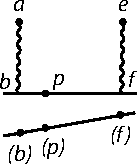
\includegraphics[width=0.16\textwidth]{gesamttex/edit_VIII,3/images/LH_35_09_16_019_d2.pdf}}% \hspace*{55mm}
  \vspace{0.5em}%
  \centerline{\lbrack\textit{Fig.~2}\rbrack}% \hspace*{55mm}
  \label{LH_35_09_16_019v_Fig.2}%
\newpage
\pstart
\noindent natura\protect\index{Sachverzeichnis}{natura} habeat libertatem eligendi,\protect\index{Sachverzeichnis}{libertas eligendi}
eliget maxime determinatum,
seu centrum gravitatis\protect\index{Sachverzeichnis}{centrum gravitatis}
descendet in linea recta,
adeoque \textit{p(p)} erit horizonti\protect\index{Sachverzeichnis}{horizon}
%
\edtext{perpendicularis,}{%
\lemma{\textit{Oberhalb} perpendicularis:}\Afootnote{%
(+\protect\vphantom)~%
forte in hoc error\protect\index{Sachverzeichnis}{error}\lbrack;\rbrack\
vide finem\textsuperscript{\lbrack a\rbrack}\!%
~+\protect\vphantom()\vspace{-0.5em}%
\newline%
\newline%
{\footnotesize%
\textsuperscript{\lbrack a\rbrack}~vide finem: S.~\refpassage{LH_35_09_16_019v_videfinem-1}{LH_35_09_16_019v_videfinem-2}.\vspace{-6mm}}}}
%
adeoque recta \textit{p(p)} \makebox[1.0\textwidth][s]{erit maxima\protect\index{Sachverzeichnis}{recta maxima}
quae esse potest.
His adjungo pondus non longius nunc esse descensurum}
\protect\index{Sachverzeichnis}{pondus pendens}\protect\index{Sachverzeichnis}{pondus tendens}
quam ante cum esset in medio,
est enim eadem vis,\protect\index{Sachverzeichnis}{vis tendens}
eademque resistentia\protect\index{Sachverzeichnis}{resistentia funis}%
\lbrack;\rbrack\
ideo non major effectus in agente\protect\index{Sachverzeichnis}{agens}%
\protect\index{Sachverzeichnis}{effectus in agente}
quemadmodum non major effectus in patiente.\protect\index{Sachverzeichnis}{patiens}%
\protect\index{Sachverzeichnis}{effectus in patiente}
Datur ergo punctum \textit{(p)}.
Quaeritur quomodo \textit{(b)(p)(f)} ducenda sit,
ut $\textit{a(b)} + \textit{e(f)}$ aequetur quantitati datae,
id quidem fiet si horizontaliter descendat trabs,\protect\index{Sachverzeichnis}{trabs}
sed videndum jam an idem fieri possit alio modo,
et quis sit ille quo discrimen inter \textit{a(b)} et \textit{e(f)} introducitur maximum.
Si ergo centro \textit{(p)} radio \textit{pb}
describatur arcus circuli\protect\index{Sachverzeichnis}{arcus circuli}
ex parte \textit{(b)},
et centro \textit{(p)} radio \textit{pf}
arcus circuli\protect\index{Sachverzeichnis}{arcus circuli}
ex parte \textit{(f)},
et ab unius circuli ad alterius circumferentiam\protect\index{Sachverzeichnis}{circumferentia circuli}
per \textit{(p)} centrum commune\protect\index{Sachverzeichnis}{centrum commune}
ducatur recta,
quaeritur quomodo illa sit
%
\edtext{ducenda \textit{(b)(p)(f)},
ut summa}{%
\lemma{ducenda}\Bfootnote{%
\textit{(1)}~, ut summa
\textit{(2)}~\textit{(b)(p)(f)}, ut summa%
~\textit{L}}}
%
$\textit{a(b)} + \textit{e(f)}$ existente data,
sit differentia earum omnium possibilium maxima.
Cum autem problema sit determinatum\protect\index{Sachverzeichnis}{problema determinatum}
ex solo dato puncto \textit{(p)}
et data recta \textit{bpf}
et data summa $\textit{a(b)} + \textit{e(f)},$
% \lbrack\textendash\rbrack\
tantum enim opus rectam \textit{bpf} circa centrum \textit{(p)} moveri
quo motu incidet
%
\edtext{in quaesita puncta,}{%
\lemma{in}\Bfootnote{%
\textit{(1)}~inf
\textit{(2)}~casus
\textit{(3)}~quaesita puncta,%
~\textit{L}}}
%
% \lbrack\textendash\rbrack\
et cum linea motus\protect\index{Sachverzeichnis}{linea motus} sit unius dimensionis,
solutiones\protect\index{Sachverzeichnis}{solutio} non possunt esse infinitae
sed casus addita conditione\protect\index{Sachverzeichnis}{conditio determinans} summae, est
%
\edtext{determinatus.\protect\index{Sachverzeichnis}{casus determinatus}
\newline%
\indent%
\edlabel{LH_35_09_16_019v_videfinem-1}%
Verum nova}{%
\lemma{determinatus.}\Bfootnote{%
\textit{(1)}~Sed addend
\textit{(2)}~Verum nova%
~\textit{L}}}
%
hic incidit consideratio\protect\index{Sachverzeichnis}{consideratio}
quod circa centrum \textit{(p)} funes
quasi vectes\protect\index{Sachverzeichnis}{vectis} collectentur.
Ergo ut sint in aequilibrio\protect\index{Sachverzeichnis}{aequilibrium}
%
\edtext{vires\protect\index{Sachverzeichnis}{vis tendens} seu tensiones\protect\index{Sachverzeichnis}{tensio} debent}{%
\lemma{vires}\Bfootnote{%
\textit{(1)}~debent
\textit{(2)}~seu tensiones debent%
~\textit{L}}}
%
esse reciproce ut distantiae a centro.\protect\index{Sachverzeichnis}{centrum}
Idem est si plures funes.\protect\index{Sachverzeichnis}{funis}
Res ergo determinata per hoc,\protect\index{Sachverzeichnis}{res determinata}
etsi priori conciliari non potest.
Non utique necesse est ut \textit{p(p)} sit perpendicularis.%
\edlabel{LH_35_09_16_019v_videfinem-2}
\edtext{Sequitur NB \astrosun\ in pag. praecedenti.}{%
\lemma{Sequitur \lbrack...\rbrack\ praecedenti}\Cfootnote{%
Siehe die Randbemerkung auf S.~\pageref{LH_35_09_16_019r_rndbmrkg_NBsun}.}}
\pend%
%
%
%  \newpage
    \count\Bfootins=1200
\count\Afootins=1200
\count\Cfootins=1200
%  \vspace{1.5em}%
%
%
%	ENDE DES STÜCKS AUF BLATT 19v.